\documentclass{article}
\usepackage{xeCJK} % 中文支持
\usepackage{fontspec} % 字体设置
\setCJKmainfont{SimSun} % 设置中文主字体
\setmainfont{Times New Roman} % 设置英文主字体

\usepackage{polyglossia} % 语言支持
\setdefaultlanguage{english}
\setotherlanguages{japanese, chinese}

\usepackage{graphicx} % 图片
\usepackage{caption}  % 用于美化标题

% % 脚注
% \usepackage{mpfnmark}
% \usepackage{fancyhdr}
% \usepackage[savemap]{footnote}

% \pagestyle{fancy}
% \fancyhf{} % 清除默认的页眉和页脚

% % 在页脚中添加脚注内容
% \fancyfoot[C]{%
%   \vspace{1em}%
%   \footnotesize%
%   \rule{\textwidth}{0.4pt}\\ % 分隔线
%   \Footnotetexts%
% }

\linespread{1.25} % 行距

% 日文支持
\newfontfamily\japanesefont{MS Mincho}
\newcommand{\jp}[1]{{\japanesefont #1}}

\begin{document}

\tableofcontents % 生成目录
\newpage

\section{入境之前}
使用iPhone设备在钱包(Wallet)中添加Suica(即俗称的西瓜卡), 可以通过Apple Pay从国内银行卡直接充值,准备一张NFC西瓜卡极其重要。(安卓系统操作方式不知道捏)\par
现在入境申报已经电子化,在入境之前事先准备QR码可以极大加速入境流程。另外,最好不要带100万以上的日元现金在身上,需要额外申报,很麻烦。\par
下载Google Map,下载Google Map,下载Google Map!
\section{行:行こうよ!}
\subsection{机场}
东京一共有两个机场:羽田(はねだ,haneda)机场和成田(なりだ,nanida)机场,地理位置都相对远离市区。因为汉字和读音接近的缘故,两个机场很容易弄混,出发前请务必确认清楚(不要问我是怎么知道的)。\par
由于羽田是新机场,所以一般是相对高价的航班,且羽田机场结构相对紧凑,例如单轨电车站与到达大厅直接相连,而在成田需要走的路就比较多了,但是成田机场航站楼之间的通道是宝可梦题材的装修(成田上大分)。\par
两个机场都有电车直通山手线的车站(山手线的战略意义见后文),其中成田机场的电车是京成電鉄运营的天空快线(スカイライナー,sukairainaa),直达日暮里(にっぽり,nippori)站:
\begin{figure}[h!]
    \centering
    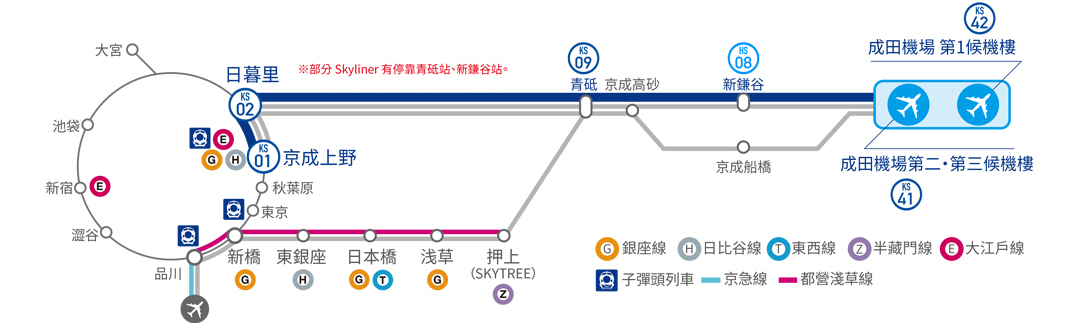
\includegraphics[width=0.9\textwidth]{./fig/routemap_skyliner.jpg} % 替换为您的图片文件
    \caption{天空快线(スカイライナー)线路图\protect\footnotemark}
\end{figure}
\footnotetext{来源:https://www.keisei.co.jp/keisei/tetudou/skyliner/jp/index.php}

羽田机场则是单轨电车(モノレール)连接的则是浜松町(はままつちょう,hamamatucyou)站:
\begin{figure}[h!]
    \centering
    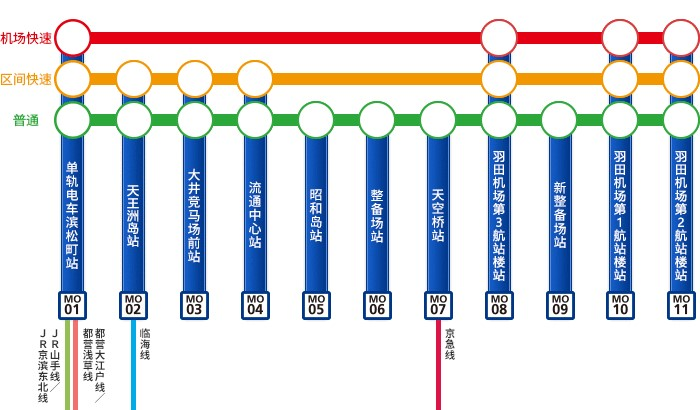
\includegraphics[width=0.6\textwidth]{./fig/routemap_monorail.jpg} % 替换为您的图片文件
    \caption{单轨电车(モノレール)线路图\protect\footnotemark}
\end{figure}
\footnotetext{来源:https://www.tokyo-monorail.co.jp/sc/guidance/index.html}

P.S.\par
全日空(ANA)在羽田有专门的check in区域。\par
两个机场都有大巴车通往包括富士山在内的各种重要地方,但是我没坐过,pass。

\subsection{电车/地铁}
东京的铁路系统是毋庸置疑的世界第一,强到断档的那种世界第一。随之而来的是非常复杂的。


\subsection{公交车}
部分的公交车是根据起落站点收费的,需要上车的时候与司机说明目的地。
日本的公交车司机会全程播报行驶状况,停车、拐弯甚至变道都要说一遍。
公交车的起步价一般略低于电车和地铁,但是,依然是100日元以上起步的。

\subsection{出租车}
在东京坐出租车的大户人家,请V我50看看实力。

\section{吃:食べましょう!}
\subsection{拉面}
为了方便,我把そば也归类到拉面里。在新宿西口旁有一家\label{res:a}。

\subsection{寿司}
在吃过100日元一贯的日本寿司郎(スシロー,sushiroo)后,对国内几乎所有的低价寿司店再没有任何兴趣。拜某位逆天日本高中生所赐,现在日本各大寿司店已经没有回转寿司这一形式了。\par
个人最喜欢的寿司店是上野附近御徒町(おかちまち,okachimachi)站前的大江户寿司。一个很多本地人都会光顾的回转寿司店。金枪鱼中腹的那种回甘令人难以忘记,关键是才250日元一贯。\par
正宗的おまさけ的聚集地之一当然是银座(ぎんざ、ginza),个人尝试过よこ田的一万日元套餐,一共14贯包含炸虾天妇罗,吃得挺饱的,但是建议这种级别的寿司只作体验即可。

\subsection{肉}

\subsection{快餐}
日本的麦当劳不支持微信支付(统计范围:东京),但是肯德基可以。\par
麦当劳没有板烧鸡腿堡、麦辣鸡腿堡这些大陆特供产品,但是。另外麦当劳的薯条默认非常咸,但是可以选择少盐。
肯德基则是完全不推荐,炸鸡非常干涩,明明日本的本土炸鸡就做得很鲜美多汁,可K记反而水平很差(但是生意却不是很差,更匪夷所思了)。

\section{山手线}
\subsection{新宿}
据说有102个出口的世界最复杂电车站就是传说中的新宿(しんじゅく,shinjuku)JR站。也许新宿不是东京人的生活中心,但是新宿往往会是在东京的游客的中心。
新宿旁边的拉面店(见\ref{res:a})。


\subsection{上野}
上野是东京的“北大门”。\par
上野最重要的设施之一便是

\subsection{东京}
在皇宫和银座之间集齐了丸之内(まるのうち,marunouchi)\par
新宿是出口最多的电车站,东京站则是最大的电车站,也是所有铁路交通方式的枢纽。东京站的面积过于大,以至于站内换乘都要接近20分钟的步行路程。\par
冷知识:丸之内线是唯一在东京站内的地铁站。\par
有乐町(ゆうらくちょ,yuurakucyo)。

\subsection{秋叶原}

\subsection{日暮里}

\subsection{池袋}

\subsection{涩谷}
首先,涩谷(しぶや,shibuya)不是“涉谷”,这是由于日语的渋长得像中文的涉而导致一个常见typo。\par
涩谷是东京几大商业中心之一,其中最知名的商场之一便是涩谷parco,七楼是常驻的任天堂商店。
实际上,明治神宫与涩谷很近,步行在20分钟以内。

\section{山手线之外}

\subsection{练马}
一开始是因为《四月是你的谎言》的取景地,我才去了練馬(ねりまく,nerimaku)。但是非常意外的,练马作为赏樱地也非常值回票价。

\subsection{日本桥}

\subsection{奥多摩}
奥多摩(おくたま,okutama),一座坐落在东京西边的村镇,一个可以洗净心灵的地方。虽然这里到东京城区需要三个小时以上的电车而且一天只有个位数电车班次,但是,这里属于东京。虽然这里几乎没有任何城市气息,路旁的树枝会伸到电车车窗里,但是,这里属于东京。(蒸馍,你不服气吗?)

\subsection{富士山}
去富士山几乎是不需要任何推荐。但是去富士山最重要的是:看天气!一定要提前查好天气。

\subsection{浅草}

\subsection{六本木}
老牌商业中心之一,观景平台。

\subsection{本乡}
东京大学

\subsection{京叶线沿途}
葛西临海公园

\subsection{横滨}

\subsection{北海道}
除了冬天去看雪,北海道并没有什么值得一去的理由,可是偏偏这个理由便已经足够说服一个人去北海道。北海道的雪景并不是多么壮丽,但是胜在氛围。另外冬季的北海道并没有同纬度其他地方那么寒冷,温度一般也就略低于0摄氏度。\par
札幌(さっぽろ,sapporo)站上便是T32观景台,在这里看札幌的夜景很出名,但是札幌并不是一个夜景多么出众的城市,与其作为一个景点不如说是来都来了顺便看看的打卡地,相对东京的几大观景台胜在人少,晚上灯光会开得很暗,氛围比东京的几大观景台更宁静。\par
如果来北海道只来札幌(就像我一样)那会损失许多宝贵的体验,但是离开札幌后在小樽和函馆的公共交通都并不发达,甚至可以说相当落后,准备出发之前需要做好充足的交通规划,可不能像在东京一样跟着电车畅玩全城。\par
我在札幌看雪的地方仅去过中岛公园。

\section{其他}
在东京的电梯靠左(大阪靠右,京都又靠左,没有什么规律可言),虽然官方已经在劝阻不要这么做,但你会见到几乎每个人都站单边,这就是空气的力量!

\section*{测试文本 テスト}
这是一段中文文本。\par
\jp{これは日本語の文章です}あいうえお。\par
This is a paragraph in English.


\end{document}